\documentclass[tikz,border=5pt]{standalone}

\usepackage{libertinus}
\usepackage{tikz}
\usepackage{pgfplots}
\pgfplotsset{compat=1.18}

\begin{document}

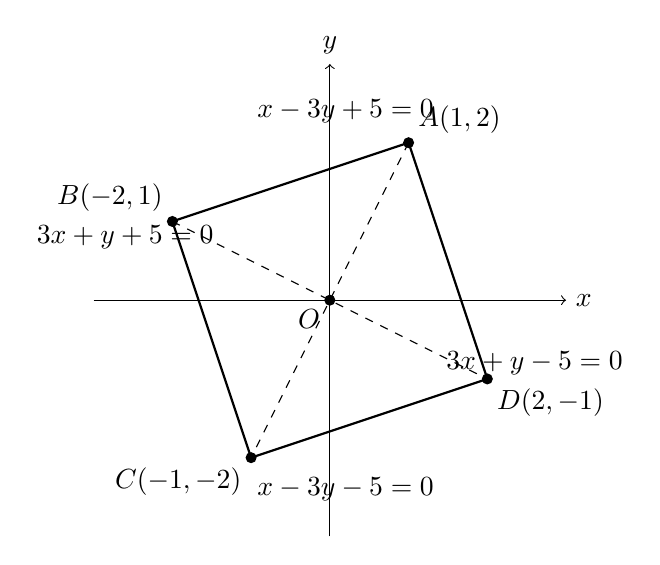
\begin{tikzpicture}[scale=1]

  % Axes
  \draw[->] (-3,0) -- (3,0) node[right] {$x$};
  \draw[->] (0,-3) -- (0,3) node[above] {$y$};

  % Vertices
  \coordinate (A) at (1,2);
  \coordinate (B) at (-2,1);
  \coordinate (C) at (-1,-2);
  \coordinate (D) at (2,-1);
  \coordinate (O) at (0,0);

  % Square
  \draw[thick] (A) -- (B) -- (C) -- (D) -- cycle;

  % Diagonals (optional visual aid)
  \draw[dashed] (A) -- (C);
  \draw[dashed] (B) -- (D);

  % Axes labels
  \fill (O) circle (2pt) node[below left] {$O$};

  % Points
  \fill (A) circle (2pt) node[above right] {$A(1,2)$};
  \fill (B) circle (2pt) node[above left] {$B(-2,1)$};
  \fill (C) circle (2pt) node[below left] {$C(-1,-2)$};
  \fill (D) circle (2pt) node[below right] {$D(2,-1)$};

  % Side labels
  \node at (0.2,2.4) {$x-3y+5=0$};
  \node at (-2.6,0.8) {$3x+y+5=0$};
  \node at (0.2,-2.4) {$x-3y-5=0$};
  \node at (2.6,-0.8) {$3x+y-5=0$};

\end{tikzpicture}

\end{document}
